\newpage
\begin{Pro}
Para los siguientes DFA obten el DFA mínimo:
\end{Pro}
\begin{enumerate}
\item 
Primero iniciamos con dos grupos, los estados de aceptacion y los estados que no son de aceptacion.

\begin{center}
\begin{align*}
    G_1 &= \{q_0\} && \text{Finales} \\
    G_2 &= \{q_1, q_2, q_3, q_4\} && \text{No finales}
\end{align*}
\end{center}

Como $G_1$ tiene un solo estado, es consistente y seguimos. 
Ahora revisamos el grupo de mayor consistencia en $G_2$. 


\begin{center}
\begin{tabular} {|c|c|c|}
    \hline
    $G_2$ & $a$ & $b$ \\ 
    \hline
    $q_1$ & $q_2 \in G_2$ & $\emptyset$ \\
    $q_2$ & $q_3 \in G_2$ & $\emptyset$ \\
    $q_3$ & $q_4 \in G_2$ & $q_0 \in G_1$ \\
    $q_4$ & $q_3 \in G_2$ & $q_0 \in G_1$ \\
    \hline
\end{tabular}
\end{center}

Dividimos $G_2$ en dos grupos nuevos, $G_2 = \{q_1, q_2\}$ y $G_3 = \{q_3, q_4\}$.

\begin{center}
\begin{tabular} {|c|c|c|}
    \hline
    $G_2$ & $a$ & $b$ \\ 
    \hline
    $q_1$ & $q_2 \in G_2$ & $\emptyset$ \\
    $q_2$ & $q_3 \in G_3$ & $\emptyset$ \\
    \hline
\end{tabular}
\end{center}

Vemos que $G_2$  no es consistente así que lo volvemos a dividir en $G_2 = \{q_1\}$ y $G_4 = \{q_2\}$.

\begin{center}
\begin{tabular} {|c|c|c|}
    \hline
    $G_3$ & $a$ & $b$ \\ 
    \hline
    $q_3$ & $q_4 \in G_3$ & $q_0 \in G_1$ \\
    $q_4$ & $q_3 \in G_3$ & $q_0 \in G_1$ \\
    \hline
\end{tabular}
\end{center}

Este grupo es consistente, por lo que ya no se puede dividir mas. Entonces los grupos finales son:

\begin{center}
\begin{align*}
    G_1 &= \{q_0\} && \text{Finales} \\
    G_2 &= \{q_1\} && \text{No finales} \\
    G_3 &= \{q_3, q_4\} && \text{No finales} \\
    G_4 &= \{q_2\} && \text{No finales}
\end{align*}
\end{center}

El DFA mínimo es:

\begin{center}
\begin{tabular} {|c|c|c|}
    \hline
    Estado    & $a$ & $b$ \\
    \hline
    $G_1$ & $q_1 \in G_2$ & $q_2 \in G_4$ \\ 
    $G_2$ & $q_2 \in G_4$ & $\emptyset$ \\
    $G_4$ & $q_3 \in G_3$ & $\emptyset$ \\
    $G_3$ & $G_3$ & $q_0 \in G_1$ \\
    \hline
\end{tabular}
\end{center}


\begin{figure}[h!]
        \centering
        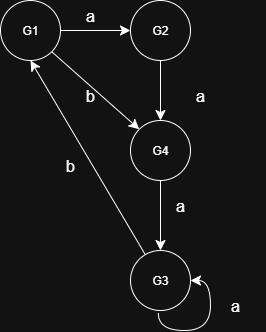
\includegraphics[width=0.4\textwidth]{images/ejercicio6a.png}
        \caption{DFA mínimo, ejercicio 6a}
\end{figure}
\newpage

    \item  : \\
    \begin{figure}[h!]
        \centering
        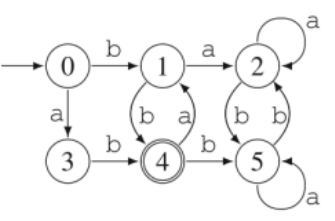
\includegraphics[width=0.5\textwidth]{images/ejercicio6b.png}
        \caption{Automata Finito Determinista, ejercicio 6 b}
    \end{figure}
    Separemos nuestros estados en dos grupos: los estados de aceptación y los que no lo son.
    \begin{itemize}
        \item Grupo 1 (aceptación): $\{q_4\}$
        \item Grupo 2 (no aceptación): $\{q_0, q_1, q_2, q_3, q_5\}$
    \end{itemize}
\newpage
    Veamos como se comportarían los estados del Grupo 2 con las entradas posibles:\\
    \begin{table}[h!]
    \centering
    \begin{tabular}{|c|c|c|}
    \hline
    \textbf{Estados} & \textbf{Transición con a} & \textbf{Transición con b } \\
    \hline
    $q_0$ & Grupo 1 & Grupo 1\\
    \hline
    $q_1$ & Grupo 1 & Grupo 2 \\
    \hline
    $q_2$  & Grupo 1 & Grupo 1 \\
    \hline
    $q_3$ & - & Grupo 2 \\
    \hline
    $q_5$ & Grupo 1 & Grupo 1 \\
    \hline
    \end{tabular}
    \label{tab:ejemplo}
    \end{table}


 Vamos a agrupar los estados que se comportan igual:\\
 \begin{itemize}
    \item Grupo A: $\{q_0, q_2, q_5\}$
    \item Grupo B: $\{q_1\}$
    \item Grupo C: $\{q_3\}$
 \end{itemize}
    Veamos como se comportarían los estados del Grupo A con las entradas posibles:  \\    
    \begin{table}[h!]
    \centering      
    \begin{tabular}{|c|c|c|}
    \hline
    \textbf{Estados} & \textbf{Transición con a} & \textbf{Transición con b } \\
    \hline
    $q_0$ & Grupo C & Grupo B\\     
    \hline
    $q_2$  & Grupo A & Grupo A \\       
    \hline
    $q_5$ & Grupo A & Grupo A \\    
    \hline
    \end{tabular}       
    \label{tab:ejemplo}
    \end{table}\\
    Ahora, agrupamos los estados que se comportan igual:\\
    \begin{itemize}     
        \item Grupo A1: $\{q_2, q_5\}$
        \item Grupo A2: $\{q_0\}$
        \item Grupo B: $\{q_1\}$
        \item Grupo C: $\{q_3\}$
    \end{itemize}
    Veamos como se comportarían los estados del Grupo A1 con las entradas posibles:   \\   
    \begin{table}[h!]        
    \centering      
    \begin{tabular}{|c|c|c|}        
    \hline
    \textbf{Estados} & \textbf{Transición con a} & \textbf{Transición con b } \\
    \hline
    $q_2$  & Grupo A1 & Grupo A1 \\ 
    \hline
    $q_5$ & Grupo A1 & Grupo A1 \\  
    \hline
    \end{tabular}       
    \label{tab:ejemplo} 
    \end{table}\\
    Notemos que ambos estados se comportan igual, por lo que no es posible seguir dividiendo los grupos. Por lo tanto, los grupos finales son:\\
    \begin{itemize} 
        \item Grupo A1: $\{q_2, q_5\}$
        \item Grupo A2: $\{q_0\}$
        \item Grupo B: $\{q_1\}$
        \item Grupo C: $\{q_3\}$
        \item Grupo D (aceptación): $\{q_4\}$   
    \end{itemize}
    Ahora, construimos el DFA mínimo usando estos grupos como estados: \\
    \begin{figure}[h!]
        \centering
        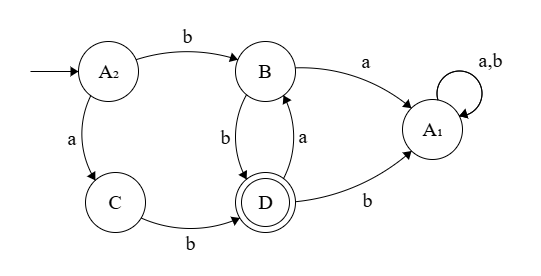
\includegraphics[width=0.5\textwidth]{images/6bresuelto.png}
        \caption{Automata Finito Determinista Minimo, ejercicio 6 b}
    \end{figure}
\end{enumerate}